\documentclass[a4paper, 11pt]{report}
\usepackage{../../preamble}
\usepackage{ amssymb }
\usepackage{tabularx}
\DeclareMathOperator{\Hessian}{Hess}

\newcommand{\rotvert}{\rotatebox[origin=c]{90}{$\vert$}}

\renewcommand{\clearpage}{}
\renewcommand{\cleardoublepage}{}
\setlength{\parindent}{0pt}

\begin{document}

\doctype{Homework}
\coursetitle{Probabilistic Graphical Models}
\semester{MVA Fall 2019}
\instructor{Pierre Latouche}
\student{Antoine Moulin, Marie Heurtevent}
\worknumber{1}
\workdate{November 22}

\maketitle

\chapter{Learning in discrete graphical models}

Consider the following model: $z$ and $x$ are discrete variables taking respectively $M$ and $K$ different values with $p(z=m) = \pi_m$ and $p(x=k|z=m) = \theta_{mk}$.

Compute the maximum likelihood estimator for $\pi$ and $\theta$ based on an i.i.d. sample of observations. Please provide your derivations and not just the final answer. \\

\textbf{Solution}. \\

Let $\left\{ (x_i, z_i) \right\}_{i \in [\![ 1, n ]\!]}$ be $n$ i.i.d. samples. The likelihood $\ell$ of $\pi \in \R^{M}$ and $\theta \in \R^{M \times K}$ is given by:

\begin{equation*}
    \begin{aligned}
    \ell \left( \pi, \theta \right) &= \ell_{(x_1, z_1), \dots, (x_n, z_n)}(\pi, \theta) \\
    &= p \left( (x_1, z_1), \dots, (x_n, z_n) | \pi, \theta \right)
    \end{aligned}
\end{equation*}
\vspace*{.6em}

By independence of the samples and by definition of the variables,

\begin{equation*}
    \begin{aligned}
    \ell \left( \pi, \theta \right) &= \prod_{i=1}^{n} p \left( x_i, z_i | \pi, \theta \right) & \text{(independence of the $(x_i, z_i)$)} \\
    &= \prod_{i=1}^{n} p \left( x_i | z_i, \pi, \theta \right) p \left( z_i | \pi, \theta \right) & \text{(definition of conditional distribution)} \\
    &= \prod_{i=1}^{n} \left( \prod_{m=1}^{M} \prod_{k=1}^{K} \theta_{mk}^{\mathds{1} \left\{ z_i = m, x_i = k \right\}} \right) \left( \prod_{m=1}^{M} \pi_{m}^{\mathds{1} \left\{ z_i = m \right\}} \right) & \text{(definition of the variables $x_i, z_i$)}
    \end{aligned}
\end{equation*}
\vspace*{.6em}

Hence, the log-likelihood $L$ is:

\begin{equation*}
    L \left( \pi, \theta \right) = \sum_{i=1}^{n} \sum_{m=1}^{M} \left( \log(\pi_m) \mathds{1}_{\left\{ z_i = m \right\}} + \sum_{k=1}^{K} \log(\theta_{mk}) \mathds{1}_{\left\{ z_i = m, x_i = k \right\}} \right)
\end{equation*}
\vspace*{.6em}

In order to get the maximum likelihood estimator for $\pi$ and $\theta$, one could maximize the log-likelihood. Hence, one has to solve the optimization problem: \\

\begin{equation*}
    \begin{aligned}
    & \min_{\pi, \theta} - L \left( \pi, \theta \right) \\
    \text{ s.t. } & \sum_{1 \leq m \leq M} \pi_{m} = 1 \\
    & \sum_{1 \leq k \leq K} \theta_{mk} = 1 \text{ for } m = 1, \dots, M
    \end{aligned}
\end{equation*}
\vspace*{.9em}

The negative log-likelihood is strictly convex with respect to $\pi$ and $\theta$. Besides, the set of feasible points is bounded and non-empty. Hence, there exists a unique minimizer for this problem. By Slater's constraint qualification, strong duality holds. For $\lambda \in \R, \mu \in \R^{M}$, the Lagrangian $\mathcal{L}$ of this problem is given by the expression:

\begin{equation*}
    \mathcal{L} \left( \pi, \theta, \lambda, \mu \right) = - L \left( \pi, \theta \right) + \lambda \left( \sum_{m=1}^{M} \pi_{m} - 1 \right) + \sum_{m=1}^{M} \mu_{m} \left( \sum_{k=1}^{K} \theta_{mk} - 1 \right)
\end{equation*}
\vspace*{.6em}

Let $m \in [\![ 1, M ]\!], k \in [\![ 1, K ]\!]$. One has:

\begin{equation*}
    \begin{aligned}
    \frac{\partial \mathcal{L}}{\partial \pi_{m}} = 0 &\text{ iff } - \frac{1}{\pi_m} \sum_{i=1}^{n} \mathds{1}_{\left\{ z_i = m \right\}} + \lambda = 0 \\
    &\text{ iff } \pi_m = \frac{1}{\lambda} \sum_{i=1}^{n} \mathds{1}_{\left\{ z_i = m \right\}}
    \end{aligned}
\end{equation*}

and,

\begin{equation*}
    \begin{aligned}
    \frac{\partial \mathcal{L}}{\partial \theta_{mk}} = 0 &\text{ iff } - \frac{1}{\theta_{mk}} \sum_{i=1}^{n} \mathds{1}_{\left\{ z_i = m, x_i = k \right\}} + \mu_{m} = 0 \\
    &\text{ iff } \mu_{m} = \frac{1}{\theta_{mk}} \sum_{i=1}^{n} \mathds{1}_{\left\{ z_i = m, x_i = k \right\}}
    \end{aligned}
\end{equation*}

Besides, the constraints ($\pi$ and the columns of $\theta$ sum to one) give us:

\begin{equation*}
    \begin{aligned}
    \sum_{m=1}^{M} \pi_{m} = 1 &\text{ iff } \frac{1}{\lambda} \sum_{m=1}^{M} \sum_{i=1}^{n} \mathds{1}_{\left\{ z_i = m \right\}} = 1 \\
    &\text{ iff } \lambda = \sum_{i=1}^{n} \sum_{m=1}^{M} \mathds{1}_{\left\{ z_i = m \right\}} \\
    &\text{ iff } \lambda = n
    \end{aligned}
\end{equation*}

and, for $m = 1, \dots, M$,

\begin{equation*}
    \begin{aligned}
    \sum_{k=1}^{K} \theta_{mk} = 1 &\text{ iff } \frac{1}{\mu_{m}} \sum_{k=1}^{K} \sum_{i=1}^{n} \mathds{1}_{\left\{ z_i = m, x_i = k \right\}} = 1 \\
    &\text{ iff } \mu_{m} = \sum_{i=1}^{n} \mathds{1}_{\left\{ z_i = m \right\}} \sum_{k=1}^{K} \mathds{1}_{\left\{ x_i = k \right\}} \\
    &\text{ iff } \mu_{m} = \sum_{i=1}^{n} \mathds{1}_{\left\{ z_i = m \right\}}
    \end{aligned}
\end{equation*}

Hence, the maximum likelihood estimators are 

\begin{equation*}
    \boxed{\begin{aligned}
    \forall m \in [\![ 1, M ]\!], \widehat{\pi}_m &= \frac{1}{n} \sum_{i=1}^{n} \mathds{1}_{\left\{ z_i = m \right\}} \\
    \forall m \in [\![ 1, M ]\!], \forall k \in [\![ 1, K ]\!], \widehat{\theta}_{mk} &= \frac{1}{\sum_{i=1}^{n} \mathds{1}_{\left\{ z_i = m \right\}}} \sum_{i=1}^{n} \mathds{1}_{\left\{ z_i = m, x_i = k \right\}} \end{aligned}}
\end{equation*}

\pagebreak
\chapter{Linear classification}

The files \texttt{trainA}, \texttt{trainB} and \texttt{trainC} contain samples of data $(x_n, y_n)$ where $x_n \in \R^2$ and $y_n \in \left\{ 0, 1 \right\}$ (each line of each file contains the $2$ components of $x_n$ then $y_n$). The goal of this exercise is to implement linear classification methods and to test them on the three data sets. The code should be written in R or Python. The source code should be handed in along with results. However, all the requested figures should be printed on paper or part of a pdf file which is turned in, with clear titles that indicate what the figures represent. Therefore, we recommend to write your code and report thanks to a Markdown file (in R or Python). The discussions may of course be handwritten.

\section{Generative model (LDA)}

Given the class variable, the data are assumed to be Gaussian with different means for different classes but with the same covariance matrix.

\begin{equation*}
    y \sim \text{Bernoulli} \left( \pi \right), x|y = i \sim \text{Normal} \left( \mu_{i}, \Sigma \right)
\end{equation*}

\begin{enumerate}[label=\alph*]
    \item Derive the form of the maximum likelihood estimator for this model.
    
    \item What is the form of the conditional distribution $p \left( y = 1 | x \right)$? Compare with the form of logistic regression.
    
    \item Implement the MLE for this model and apply it to the data. Represent graphically the data as a point cloud in $\R^{2}$ and the line defined by the equation
    
    \begin{equation*}
        p \left( y = 1 | x \right) = 0.5
    \end{equation*}
\end{enumerate}

\textbf{Solution.} \\

\begin{enumerate}[label=\alph*]
    \item Let $\left\{ (x_k, y_k) \right\}_{k \in [\![ 1, n ]\!]}$ be $n$ i.i.d. samples. We note that $\Sigma$ has to be positive definite, otherwise the density would not be defined. As in the first part, using the independence of the samples and the definition of the variables, one can show that the likelihood of $\theta = \left( \pi, \mu_{0}, \mu_{1}, \Sigma \right)$ is given by:
    
    \begin{equation*}
        \begin{aligned}
        \ell \left( \theta \right) &= p \left( \left( x_1, y_1 \right), \dots, \left( x_n, y_n \right) | \theta \right) & \\
        &= \prod_{k=1}^{n} p \left( x_k, y_k | \theta \right) \\
        &= \prod_{k=1}^{n} p \left( x_k | y_k, \theta \right) p \left( y_k | \theta \right) \\
        &= \prod_{k=1}^{n} \left( \frac{1}{\left( 2 \Pi \right)^{d/2} \left| \Sigma \right|^{1/2}} \exp \left[ - \frac{1}{2} \left( x_k - \mu_{y_k} \right)^{T} \Sigma^{-1} \left( x_k - \mu_{y_k} \right) \right] \right) \left( \pi^{y_k} \left( 1 - \pi \right)^{1-y_k} \right)
        \end{aligned}
    \end{equation*}
    \vspace*{.6em}
    
    where $d = 2$ is the dimension of the $x_k$'s and $\Pi$ the universal constant (not to be confused with the parameter $\pi$). Hence, the log-likelihood $L$ is given by:
    
    \begin{equation*}
        \begin{aligned}
        L \left( \theta \right) = - \frac{nd}{2} \log 2 \Pi - \frac{n}{2} \log \left| \Sigma \right| + \sum_{k=1}^{n} \left\{ - \frac{1}{2} \left( x_k - \mu_{y_k} \right)^{T} \Sigma^{-1} \left( x_k - \mu_{y_k} \right) + y_{k} \log \left( \pi \right) + \left( 1 - y_{k} \right) \log \left( 1 - \pi \right) \right\}
        \end{aligned}
    \end{equation*}
    
    $L$ is differentiable. Let's compute the gradient with respect to $\pi, \mu_{0}, \mu_{1}$ and $\Sigma$. We have:
    
    \begin{equation*}
        \begin{aligned}
        \frac{\partial L}{\partial \pi} &= \frac{1}{\pi} \sum_{k=1}^{n} y_{k} - \frac{1}{1 - \pi} \sum_{k=1}^{n} 1 - y_{k} \\
        &= \frac{1}{\pi} \sum_{k=1}^{n} y_{k} - \frac{1}{1 - \pi} \left( n - \sum_{k=1}^{n} y_{k} \right)
        \end{aligned}
    \end{equation*}
    
    Hence, 
    
    \begin{equation*}
        \begin{aligned}
        \frac{\partial L}{\partial \pi} = 0 &\text{ iff } \frac{1}{\pi} \sum_{k=1}^{n} y_{k} = \frac{1}{1 - \pi} \left( n - \sum_{k=1}^{n} y_{k} \right) \\
        &\text{ iff } \pi = \frac{1}{n} \sum_{k=1}^{n} y_{k} \\
        &\text{ iff } \pi = \frac{n_{1}}{n} \triangleq \widehat{\pi}
        \end{aligned}
    \end{equation*}
    
    where $n_{1} = \sum_{k=1}^{n} y_{k} = \sum_{k=1}^{n} \mathds{1}_{\left\{ y_{k} = 1 \right\}}$ (we also define $n_{0} = \sum_{k=1}^{n} \mathds{1}_{\left\{ y_{k} = 0 \right\}} = n - n_{1}$). The MLE estimator for $\pi$ is the proportion of examples from the class $1$ in the dataset. Now, the gradient with respect to $\mu_{i}$, where $i \in \left\{ 0, 1 \right\}$, is
    
    \begin{equation*}
        \begin{aligned}
        \frac{\partial L}{\partial \mu_{i}} = \Sigma^{-1} \sum_{k=1}^{n} \left( x_{k} - \mu_{i} \right) \mathds{1}_{\left\{ y_k = i \right\}}
        \end{aligned}
    \end{equation*}
    
    It is zero when
    
    \begin{equation*}
        \begin{aligned}
        \frac{\partial L}{\partial \mu_{i}} = 0 &\text{ iff } \sum_{k=1}^{n} \left( x_{k} - \mu_{i} \right) \mathds{1}_{\left\{ y_{k} = i \right\}} = 0 \\
        &\text{ iff } \mu_{i} = \frac{1}{n_{i}} \sum_{k=1}^{n} x_{k} \mathds{1}_{\left\{ y_{k} = i \right\}} \triangleq \widehat{\mu}_{i}
        \end{aligned}
    \end{equation*}
    
    Hence, the MLE estimator for $\mu_{i}$ is the empirical mean relatively to the class $i$. The gradient of $L$ with respect to $\Sigma$ is equal to the gradient of $g: \Sigma \mapsto - \frac{n}{2} \log \left| \Sigma \right| - \frac{1}{2} \sum_{k=1}^{n} \left( x_{k} - \widehat{\mu}_{y_{k}} \right)^{T} \Sigma^{-1} \left( x_{k} - \widehat{\mu}_{y_{k}} \right)$. Note that we replace the $\mu_{i}$ by their estimator $\widehat{\mu}_{i}$. As the second term is a sum of real numbers, one can write:
    
    \begin{equation*}
        \begin{aligned}
        g \left( \Sigma \right) &= - \frac{n}{2} \log \left| \Sigma \right| - \frac{1}{2} \sum_{k=1}^{n} \Tr \left[ \left( x_{k} - \widehat{\mu}_{y_{k}} \right)^{T} \Sigma^{-1} \left( x_{k} - \widehat{\mu}_{y_{k}} \right) \right] \\
        &= - \frac{n}{2} \log \left| \Sigma \right| - \frac{1}{2} \sum_{k=1}^{n} \Tr \left[ \Sigma^{-1} \left( x_{k} - \widehat{\mu}_{y_{k}} \right) \left( x_{k} - \widehat{\mu}_{y_{k}} \right)^{T} \right] \\
        &= - \frac{n}{2} \left( \log \left| \Sigma \right| + \Tr \left( \Sigma^{-1} \Tilde{\Sigma} \right) \right)
        \end{aligned}
    \end{equation*}
    
    where $\Tilde{\Sigma} = \frac{1}{n} \sum_{k=1}^{n} \left( x_{k} - \widehat{\mu}_{y_{k}} \right) \left( x_{k} - \widehat{\mu}_{y_{k}} \right)^{T}$ is the empirical covariance matrix. 
    
    \underline{Derivative of the first term of $g$}. Let's compute the gradient of the function $X \in \cS_{++}^{n} \left( \R \right) \longmapsto \log \left| X \right|$. For $X, H \in \cS_{++}^{n} \left( \R \right)$ such that $H$ is small (e.g. its Frobenius norm is small), one has:
    
    \begin{equation*}
        \begin{aligned}
        \log \det \left( X + H \right) &= \log \det \left[ X^{1/2} \left( I + X^{-1/2}HX^{-1/2} \right) X^{1/2} \right] \\
        &= \log \det X + \log \det \left( I + X^{-1/2}HX^{-1/2} \right) \\
        &= \log \det X + \sum_{i=1}^{n} \log \left( 1 + \lambda_{i} \right)
        \end{aligned}
    \end{equation*}
    \vspace*{.6em}
    
    where $\lambda_{i}$ is the $i$-th eigenvalue of $X^{-1/2}HX^{-1/2}$. $H$ is small, so are its eigenvalues. Hence, one can make the first-order approximation $\log \left( 1 + \lambda_{i} \right) = \lambda_{i} + \underset{\lambda_{i} \rightarrow 0}{o} \left( \lambda_{i} \right)$, which gives:
    
    \begin{equation*}
        \begin{aligned}
        \log \det \left( X + H \right) &= \log \det X + \Tr \left( X^{-1/2}HX^{-1/2} \right) + \underset{\norm{H}{} \rightarrow 0}{o} \left( H \right) \\
        &= \log \det X + \Tr \left( X^{-1} H \right) + \underset{\norm{H}{} \rightarrow 0}{o} \left( H \right)
        \end{aligned}
    \end{equation*}
    
    Because, $X^{-1}$ is symmetric, the second term corresponds to the Frobenius inner product between $X^{-1}$ and $H$. It is possible to identify the gradient of this function with respect to $X$: it is equal to $X^{-1}$.
    
    \underline{Derivative of the second term of $g$}. Let's compute the gradient of $X \in \cS_{++}^{n} \left( \R \right) \longmapsto \Tr \left( X^{-1} \Tilde{\Sigma} \right)$. For $X, H \in \cS_{++}^{n} \left( \R \right)$ such that $H$ is small (for $I + X^{-1}H$ to be invertible, it is supposed small enough so that $\norm{X^{-1}H}{} < 1$ holds), one has:
    
    \begin{equation*}
        \begin{aligned}
        \Tr \left[ \left( X + H \right)^{-1} \Tilde{\Sigma} \right] &= \Tr \left[ \left( I + X^{-1}H \right)^{-1} X^{-1} \Tilde{\Sigma} \right]
        \end{aligned}
    \end{equation*}
    
    Because $\norm{X^{-1}H}{} < 1$ (and $\norm{\cdot}{}$ a sub-multiplicative norm), one has:
    
    \begin{equation*}
        \left( I + X^{-1}H \right)^{-1} = \sum_{k=0}^{+ \infty} \left( -1 \right)^{k} \left( X^{-1}H \right)^{k}
    \end{equation*}
    
    which gives:
    
    \begin{equation*}
        \begin{aligned}
        \Tr \left[ \left( X + H \right)^{-1} \Tilde{\Sigma} \right] &= \underbrace{\Tr \left( X^{-1}\Tilde{\Sigma} \right)}_{k=0} + \underbrace{\Tr \left[ - X^{-1}HX^{-1} \Tilde{\Sigma} \right]}_{k=1} + \underbrace{\underset{\norm{H}{} \rightarrow 0}{o} \left( H \right)}_{k > 2} \\
        &= \Tr \left( X^{-1}\Tilde{\Sigma} \right) + \Tr \left[ \left( - X^{-1}\Tilde{\Sigma}X^{-1} \right) H \right] + \underset{\norm{H}{} \rightarrow 0}{o} \left( H \right)
        \end{aligned}
    \end{equation*}
    
    Once again, it is possible to identify the gradient of this function with respect to $X$, which is equal to $- X^{-1}\Tilde{\Sigma}X^{-1}$ (because the matrices are symmetric).
    
    Hence, the gradient of the log-likelihood with respect to $\Sigma$ is:
    
    \begin{equation*}
        \begin{aligned}
        \frac{\partial L}{\partial \Sigma} &=  \frac{\partial g}{\partial \Sigma} \\
        &= - \frac{n}{2} \left( \Sigma^{-1} - \Sigma^{-1} \Tilde{\Sigma} \Sigma^{-1} \right)
        \end{aligned}
    \end{equation*}
    
    and we have
    
    \begin{equation*}
        \begin{aligned}
        \frac{\partial L}{\partial \Sigma} = 0 &\text{ iff } \Sigma^{-1} - \Sigma^{-1} \Tilde{\Sigma} \Sigma^{-1} = 0 \\
        &\text{ iff } \Sigma = \Tilde{\Sigma} \triangleq \widehat{\Sigma}
        \end{aligned}
    \end{equation*}
    
    This shows that the $\left( \widehat{\pi}, \widehat{\mu}_{0}, \widehat{\mu}_{1}, \widehat{\Sigma} \right)$ obtained is the only stationary point of the log-likelihood. To check that it corresponds to a maximum, one can compute the Hessian matrix. To sum up, the maximum likelihood estimators are given by:
    
    \begin{equation*}
        \boxed{\begin{aligned}
        \widehat{\pi} &= \frac{n_{1}}{n} \\        \widehat{\mu}_{i} &= \frac{1}{n_{i}} \sum_{k=1}^{n} x_{k} \mathds{1}_{\left\{ y_{k} = i \right\}} & \text{ for } i \in \left\{ 0, 1 \right\} \\
        \widehat{\Sigma} &= \frac{1}{n} \sum_{k=1}^{n} \left( x_{k} - \widehat{\mu}_{y_{k}} \right) \left( x_{k} - \widehat{\mu}_{y_{k}} \right)^{T} 
        \end{aligned}}
    \end{equation*}
    
    \item One has:
    
    \begin{equation*}
        \begin{aligned}
        p \left( y = 1 | x \right) &= \frac{p \left( x | y = 1 \right) p ( y = 1 )}{p(x | y = 0) p(y = 0) + p(x | y = 1) p(y = 1)} \\
        &= \frac{\exp \left[ - \frac{1}{2} \left( x - \mu_{1} \right)^{T} \Sigma^{-1} \left( x - \mu_{1} \right) \right] \pi}{\exp \left[ - \frac{1}{2} \left( x - \mu_{0} \right)^{T} \Sigma^{-1} \left( x - \mu_{0} \right) \right] \left( 1 - \pi \right) + \exp \left[ - \frac{1}{2} \left( x - \mu_{1} \right)^{T} \Sigma^{-1} \left( x - \mu_{1} \right) \right] \pi} \\
        &= \frac{1}{\left( \frac{1}{\pi} - 1 \right) \exp \left[ \frac{1}{2} \left\{ \left( x - \mu_{1} \right)^{T} \Sigma^{-1} \left( x - \mu_{1} \right) - \left( x - \mu_{0} \right)^{T} \Sigma^{-1} \left( x - \mu_{0} \right) \right\} \right] + 1} \\
        &= \frac{1}{\exp \left[ \frac{1}{2} \left\{ 2 \mu_{0}^{T} \Sigma^{-1} x - 2 \mu_{1}^{T} \Sigma^{-1} x + \mu_{1}^{T} \Sigma^{-1} \mu_{1} - \mu_{0}^{T} \Sigma^{-1} \mu_{0} \right\} + \ln \left( \frac{1}{\pi} - 1 \right) \right] + 1} \\
        &= \frac{1}{1 + \exp \left( -(w^{T}x + b) \right)} \\
        \end{aligned}
    \end{equation*}
    
    where $w = \Sigma^{-1} \left( \mu_{1} - \mu_{0} \right)$ because $\Sigma^{-1}$ is symmetric and $b = -\frac{1}{2} \left( \mu_{1}^{T} \Sigma^{-1} \mu_{1} - \mu_{0}^{T} \Sigma^{-1} \mu_{0} \right) + \ln \left(\frac{\pi}{1-\pi}\right)$. The first line comes from the Bayes' theorem. The second line just comes from the definition of the distributions and some simplifications. Hence, denoting $\sigma$ the sigmoid function,
    
    \begin{equation*}
        \boxed{\begin{aligned}
        p \left( y = 1 | x \right) = \sigma \left(w^{T}x + b \right) \text{ where } & w = \Sigma^{-1} \left( \mu_{1} - \mu_{0} \right) \\
        & b = -\frac{1}{2} \left( \mu_{1}^{T} \Sigma^{-1} \mu_{1} - \mu_{0}^{T} \Sigma^{-1} \mu_{0} \right) + \ln \left( \frac{\pi}{1-\pi} \right)
        \end{aligned}}
    \end{equation*}
    
    \item The MLE for this model are implemented in the Python class \texttt{LDA}, in the file \texttt{lda.py}. In the following table are the numerical values of the parameters learnt for the LDA model. \\

        \begin{tabular}{ | l || *{3}{c| } }
             \hline
                Parameter & Dataset A & Dataset B & Dataset C \\
             \hline			
               w_0 & 2.019 & 1.703 & 0.302 \\
               w_1 & -6.378 & -3.043 & -2.868 \\
               b & 31.951 & 7.886 & 20.574 \\
             \hline  
         \end{tabular}
         \vspace*{.6em}

    Besides, in figure \ref{fig:lda-plots} are shown the data as well as the line defined by $p \left( y = 1 | x \right) = 0.5$.

        \begin{figure*}[!htb]
        \minipage{0.5\textwidth}
          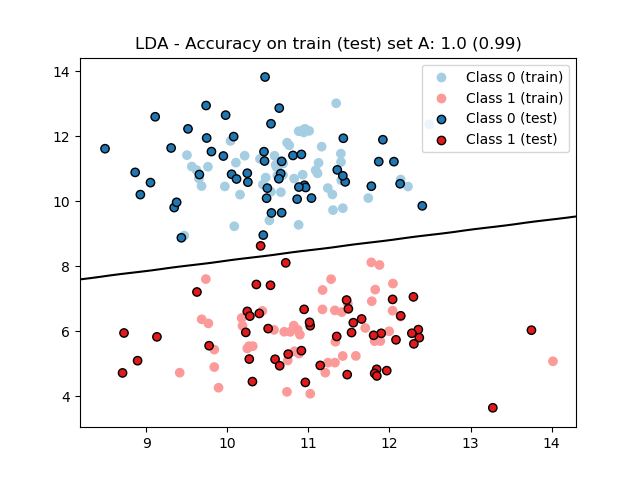
\includegraphics[width=\linewidth]{./images/LDA_A.png}
          \label{fig:lda_a}
        \endminipage\hfill
        \minipage{0.5\textwidth}
          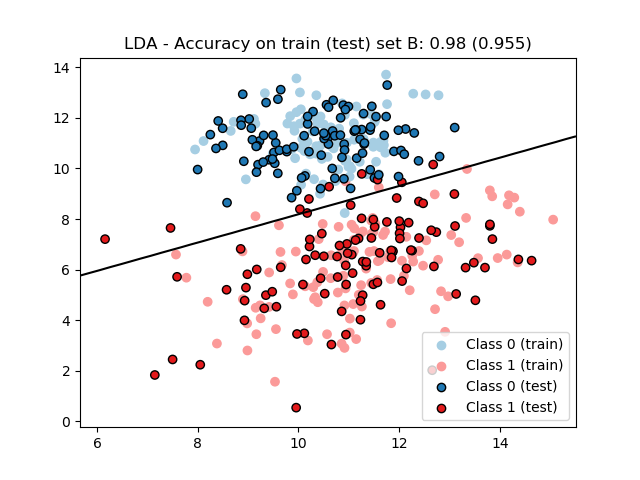
\includegraphics[width=\linewidth]{./images/LDA_B.png}
          \label{fig:lda_b}
        \endminipage\hfill
        \vspace*{-.8cm}
        \minipage{0.5\textwidth}
          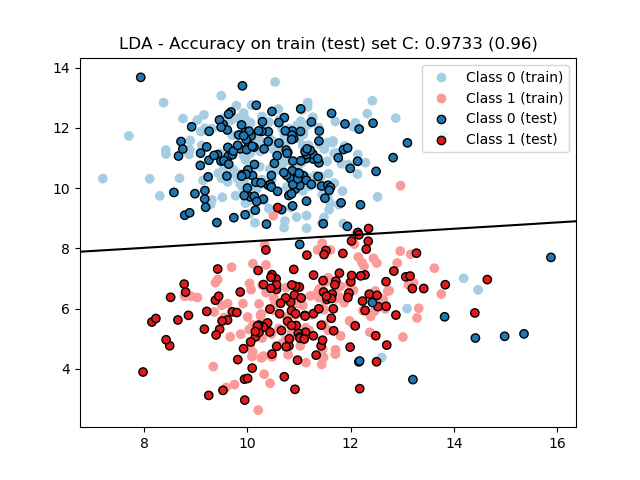
\includegraphics[width=\linewidth]{./images/LDA_C.png}
          \label{fig:lda_c}
        \endminipage
        \vspace*{-.8cm}
        \caption{The lines are defined by the equation $p(y=1|x)=0.5$ for the LDA Model.}
        \label{fig:lda-plots}
        \end{figure*}
\end{enumerate}

\section{Logistic regression}

Implement logistic regression for an affine function $f(x) = w^{T}x + b$ (do not forget the constant term).

\begin{enumerate}[label=\alph*]
    \item Give the numerical values of the parameters learnt.
    
    \item Represent graphically the data as a cloud point in $\R^{2}$ as well as the line defined by the equation
    
    \begin{equation*}
        p \left( y = 1 | x \right) = 0.5
    \end{equation*}
\end{enumerate}

\textbf{Solution.} \\

For the logistic regression, we will assume: $ y|x \sim \mathcal{B}(\theta)$, a Bernoulli law with parameter $\theta = \sigma(w^Tx) $. \\ 

In this case, the offset $b$ is incorporated in the weight vector $w$ with: $
    \left\{
        \begin{array}{ll}
            w := \quad
                    \begin{pmatrix} 
                    b \\
                    | \\
                    w \\
                    |
                    \end{pmatrix} \\
            X := \quad
                    \begin{pmatrix} 
                    1 & \protect\rotvert\; x_{1}^{T} \;\protect\rotvert \\
                    \vdots & \vdots \\
                    1 & \protect\rotvert\; x_{n}^{T} \;\protect\rotvert
                    \end{pmatrix} \\
        \end{array}
    \right.
    $ where $\left\{ \left( x_{i}, y_{i} \right) \right\}_{i \in [\![ 1, n ]\!]} \subset \R^{d} \times \left\{ 0, 1 \right\}$ are $n$ i.i.d. samples.
    
    \\ With this in mind, we find:
    \begin{equation*}
        \begin{aligned}
        p \left( y|x \right) &= \theta^y(1-\theta)^{1-y} & \\
        &= \sigma \left( w^Tx \right)^y \left( 1-\sigma \left( w^Tx \right) \right)^{1-y}
        \end{aligned}
    \end{equation*}
    \vspace*{.6em}
    
    \\ As such, the log-likelihood is given by:
    
    \begin{equation*}
        \begin{aligned}
        L \left( w \right) &= \sum_{k=1}^{n} y_k \log \sigma(w^Tx_k) + (1-y_k)\log(1 - \sigma(w^Tx_k)) \\
        &= \sum_{k=1}^{n} y_k \log \sigma(w^Tx_k) + (1-y_k)\log\sigma(-w^Tx_k)
        \end{aligned}
    \end{equation*}
    \vspace*{.6em}
    
    We can calculate the gradient since $w \mapsto w^Tx$ is linear and $z \mapsto \log \sigma(z) = - \log(1 + e^{-z}) $ is concave:
    
    \begin{equation*}
        \begin{aligned}
        \nabla_w L \left( w \right) &= \sum_{k=1}^{n} y_k \frac{ \nabla_w(\sigma(w^Tx_k)) }{\sigma(w^Tx_k)}  + (1-y_k)\frac{ \nabla_w(\sigma(-w^Tx_k)) }{\sigma(-w^Tx_k)} \\
        &= \sum_{k=1}^{n} y_k x_k \frac{ \nabla_w(\sigma)(w^Tx_k) }{\sigma(w^Tx_k)}  - (1-y_k)x_k \frac{ \nabla_w(\sigma)(-w^Tx_k) }{\sigma(-w^Tx_k)} \\
        \end{aligned}
    \end{equation*}
    \vspace*{.6em}
    
    As $\sigma'$ is given by $\sigma' = \sigma \left( 1 - \sigma \right)$,
    
    \begin{equation*}
        \begin{aligned}
        \nabla_w L \left( w \right) &= \sum_{k=1}^{n} y_k x_k \frac{ \sigma(w^Tx_k)(1 - \sigma(w^Tx_k)) }{\sigma(w^Tx_k)}  - (1-y_k)x_k \frac{ \sigma(-w^Tx_k)(1-\sigma(-w^Tx_k)) }{\sigma(-w^Tx_k)} \\
        &= \sum_{k=1}^{n} y_k x_k (1 - \sigma(w^Tx_k))  - (1-y_k)x_k \sigma(w^Tx_k) \\
        &= \sum_{k=1}^{n} x_k \left[y_k - y_k\sigma(w^Tx_k))  - \sigma(w^Tx_k) + y_k\sigma(w^Tx_k) \right]\\
        &= \sum_{k=1}^{n} x_k \left[y_k  - \sigma(w^Tx_k) \right]
        \end{aligned}
    \end{equation*}
    
    The equation $ \nabla_w L \left( w \right) = 0 \iff \sum_{k=1}^{n} x_k \left[y_k  - \sigma(w^Tx_k) \right] = 0$ is nonlinear, so we can use the Newton-Raphson method to find a good root approximation. Therefore, we need to compute the Hessian. 
    \begin{equation*}
        \begin{aligned}
        \Hessian L \left( w \right) &= \sum_{k=1}^{n} -x_k \sigma(w^Tx_k) \sigma(-w^Tx_k)x_k^T \\
        &= - X^T \Diag\left(\sigma(w^Tx_k) \sigma(-w^Tx_k)\right)X \\
        \end{aligned}
    \end{equation*}
    where The Newton-Raphson method then consists in updating $w$ as follows:
    \begin{equation*}
        \begin{aligned}
        w_{t+1} &= w_t - \Hessian L \left( w_t \right)^{-1} \nabla_w L \left(w_t\right) 
        \end{aligned}
    \end{equation*}

\begin{enumerate}[label=\alph*]
    \item In the following table are the numerical values of the parameters learnt for the Logistic Regression model. \\
    \\
        \begin{tabular}{ | l || *{3}{c| } }
             \hline
                Parameter & Dataset A & Dataset B & Dataset C \\
             \hline			
               w_0 & 16.999 & 1.842 & -0.277 \\
               w_1 & -66.605 & -3.714 & -1.914 \\
               b & 378.214 & 13.430 & 18.807 \\
            \hline
               Number of iterations & 200 & 11 & 9 \\
               Convergence & False & True & True \\
             \hline  
         \end{tabular}
    
    \item This model is implemented in the Python class \texttt{LogisticRegression}, in the file \texttt{log\_reg.py}. In the figure \ref{fig:log-reg-plot} are shown the data as well as the line defined by $p \left( y=1 | x \right) = 0.5$.
    
        \begin{figure}[!htb]
        \minipage{0.5\textwidth}
          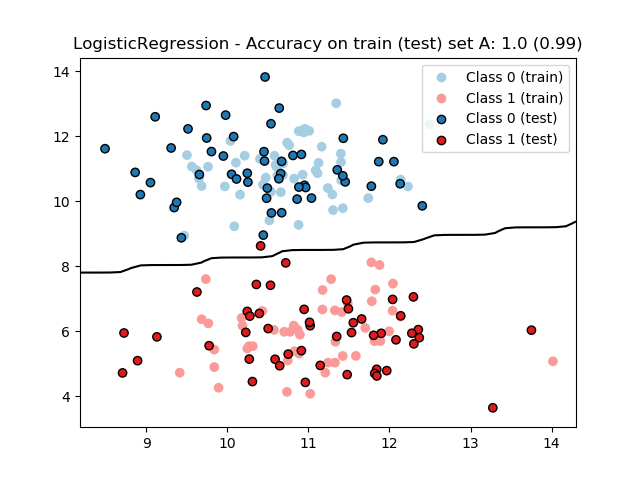
\includegraphics[width=\linewidth]{./images/LogReg_A.png}
          \label{fig:logreg_a}
        \endminipage\hfill
        \minipage{0.5\textwidth}
          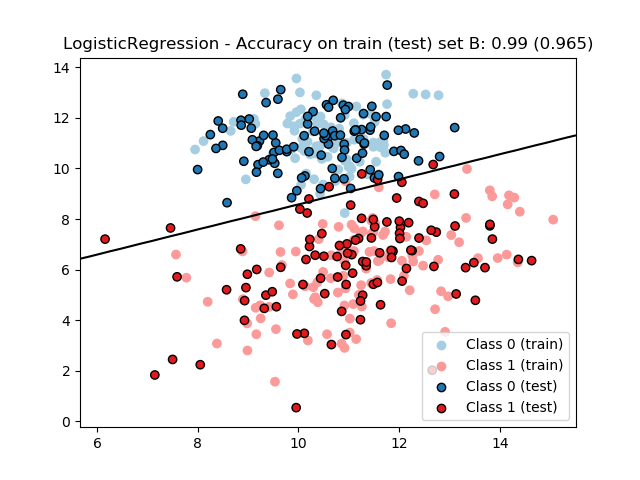
\includegraphics[width=\linewidth]{./images/LogReg_B.png}
          \label{fig:logreg_b}
        \endminipage\hfill
        \minipage{0.5\textwidth}%
          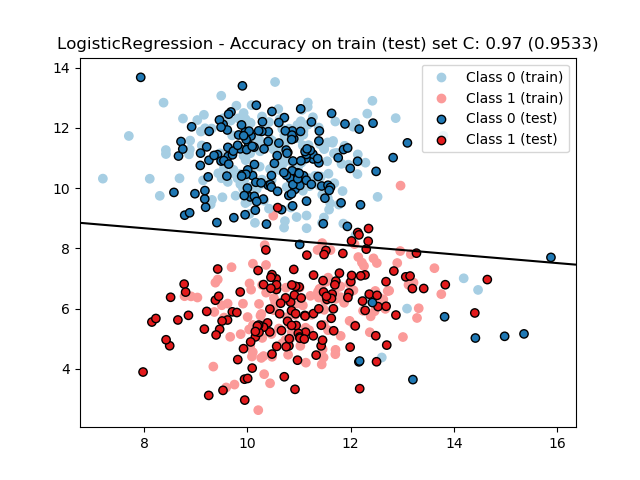
\includegraphics[width=\linewidth]{./images/LogReg_C.png}
          \label{fig:logreg_c}
        \endminipage
        \caption{The lines are defined by the equation $p(y=1|x)=0.5$ for the Logistic Regression model.}
        \label{fig:log-reg-plot}
        \end{figure}
\end{enumerate}

\section{Linear regression}

Consider class $y$ as a real valued variable taking the values $0$ and $1$ only. Implement linear regression (for an affine function $f(x) = w^{T}x + b$) by solving the normal equations.

\begin{enumerate}[label=\alph*]
    \item Provide the numerical values of the learnt parameters.
    
    \item Represent graphically the data as a point cloud in $\R^{2}$ as well as the line defined by the equation
    
    \begin{equation*}
        p \left( y = 1 | x \right) = 0.5
    \end{equation*}
\end{enumerate}

\textbf{Solution.} \\

Given a dataset $\left\{ \left( x_{i}, y_{i} \right) \right\}_{i \in [\![ 1, n ]\!]} \subset \R^{d} \times \left\{ 0, 1 \right\}$, a linear regression can be obtained solving an ordinary least squares (OLS) problem:
    
\begin{equation*}
\left( w, b \right) \in \underset{w \in \R^{d}, b \in \R}{\arg\min} \sum_{i=1}^{n} \left( y_{i} - \left( w^{T}x_{i} + b \right) \right)^{2}    
\end{equation*}

Note that this is not an equality as the solution is, \textit{a priori}, not unique. \\

Using matrices, it is equivalent to solve:
    
\begin{equation*}
    \theta \in \underset{\theta \in \R^{d+1}}{\arg\min} \norm{Y - X \theta}{2}^{2}
\end{equation*}
    
where $\theta = \left( b, w_{1}, \dots, w_{d} \right)^{T}$, $Y$ is the $n$-dimensional vector formed by the $y_{i}$'s, $X \in \R^{n \times (d+1)}$ the matrix defined by
    
\begin{equation*}
    X = \begin{pmatrix} 
            1 & \protect\rotvert\; x_{1}^{T} \;\protect\rotvert \\
            \vdots & \vdots \\
            1 & \protect\rotvert\; x_{n}^{T} \;\protect\rotvert
        \end{pmatrix}
\end{equation*}
    
The uniqueness of the solution depends on $\Ker \left( X \right)$ (if $\Ker \left( X \right) = \left\{ 0 \right\}$ it is unique, otherwise the set of solutions is given by $\widehat{\theta} + \Ker \left( X \right)$ where $\widehat{\theta}$ is a particular solution). Solving the so-called normal equation, $X^{T} \left( Y - \widehat{Y} \right) = 0$ where $\widehat{Y} = X \widehat{\theta}$ and $\widehat{\theta}$ is a particular solution, one can show that a solution is given by:
    
\begin{equation*}
    \widehat{\theta} = \left( X^{T} X \right)^{+} X^{T} Y
\end{equation*}
    
where $\left( X^{T} X \right)^{+}$ is the Moore-Penrose inverse of $X^{T} X$ (which always exists), that corresponds to the usual inverse when $X^{T} X$ is invertible.
    
\begin{enumerate}[label=\alph*]
    \item In the following table are the numerical values of the parameters learnt for the Linear Regression model. \\
    \\
        \begin{tabular}{ | l || *{3}{c| } }
             \hline
                Parameter & Dataset A & Dataset B & Dataset C \\
             \hline			
               w_0 & 0.056 & 0.083 & 0.017 \\
               w_1 & -0.176 & -0.148 & -0.159 \\
               b & 1.383 & 0.882 & 1.640 \\
             \hline  
         \end{tabular}
    
    \item The MLE for this model are implemented in the Python class \texttt{LinearRegression}, in the file \texttt{lin\_reg.py}. In the figure \ref{fig:lin-reg-plot} are shown the data as well as the line defined by $p \left( y=1 | x \right) = 0.5$.
    
        \begin{figure}[!htb]
        \minipage{0.5\textwidth}
          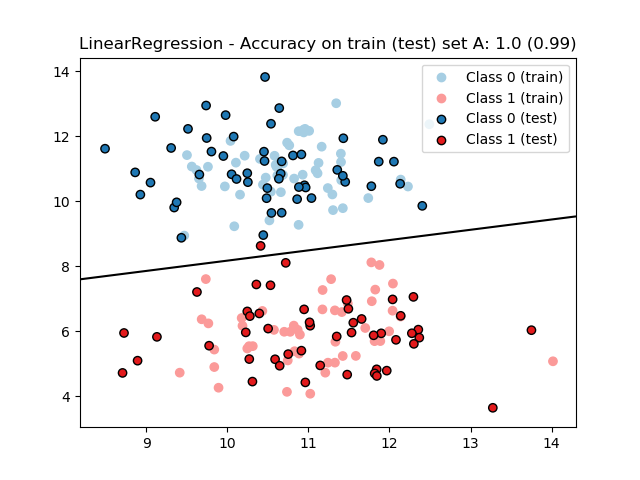
\includegraphics[width=\linewidth]{./images/LinReg_A.png}
          \label{fig:linreg_a}
        \endminipage\hfill
        \minipage{0.5\textwidth}
          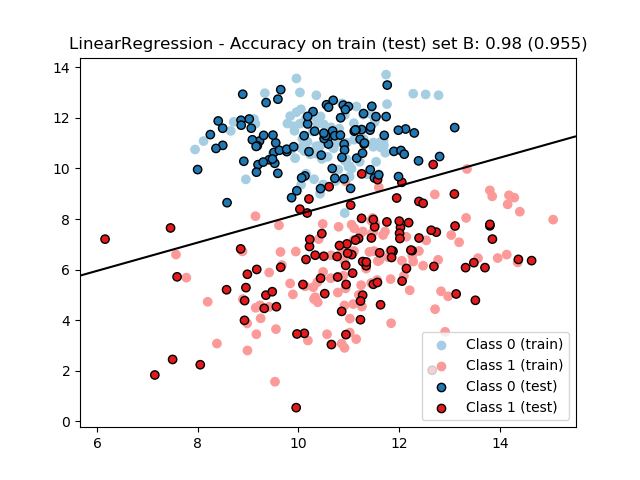
\includegraphics[width=\linewidth]{./images/LinReg_B.png}
          \label{fig:linreg_b}
        \endminipage\hfill
        \minipage{0.5\textwidth}%
          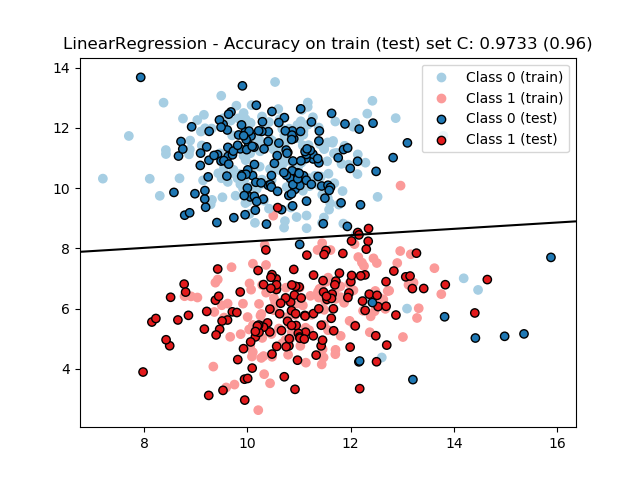
\includegraphics[width=\linewidth]{./images/LinReg_C.png}
          \label{fig:linreg_c}
        \endminipage
        \caption{The lines are defined by the equation $p(y=1|x)=0.5$ for the Linear Regression model.}
        \label{fig:lin-reg-plot}
        \end{figure}
\end{enumerate}

\section{Application}

Data in the files \texttt{testA}, \texttt{testB}, \texttt{testC} are respectively drawn from the same distribution as the data in the files \texttt{trainA}, \texttt{trainB} and \texttt{trainC}. Test the different models learnt from the corresponding training data on these test data.

\begin{enumerate}[label=\alph*]
    \item Compute for each model the misclassification error (\ie the fraction of the data misclassified) on the training data and compute it as well on the test data.
    
    \item Compare the performances of the different methods on the three datasets. Is the misclassification error larger, smaller, or similar on the training and test data? Why? Which methods yield very similar/dissimilar results? Which methods yield the best results on the different datasets? Provide an interpretation.
\end{enumerate}

\textbf{Solution.} \\

\begin{enumerate}[label=\alph*]
    \item Below are shown the misclassification errors on each dataset, for each model: \\
    
    LDA \hfill
    \begin{tabular}{ | l | *{3}{| c} | }
         \hline
            Misclassif. error & Dataset A & Dataset B & Dataset C \\
         \hline
            Train set & 0    & 0.02  & 0.027 \\
            Test set  & 0.01 & 0.045 & 0.04  \\
         \hline
     \end{tabular}
    
    Logistic Regression \hfill
    \begin{tabular}{ | l | *{3}{| c} | }
         \hline
            Misclassif. error & Dataset A & Dataset B & Dataset C \\
         \hline
           Train set & 0    & 0.01  & 0.03  \\
           Test set  & 0.01 & 0.035 & 0.047 \\
         \hline
     \end{tabular}
    
    Linear Regression \hfill
    \begin{tabular}{ | l | *{3}{| c} | }
         \hline
            Misclassif. error & Dataset A & Dataset B & Dataset C \\
         \hline
           Train set & 0    & 0.02  & 0.027 \\
           Test set  & 0.01 & 0.045 & 0.04  \\
         \hline
    \end{tabular}
    
    \item \begin{itemize}
        \item The misclassification error is always larger on the test set. On the dataset A, it is quite similar. It is due to the fact that the data is linearly separable and the points closest to the border are all in the training set except for one (hence the one misclassfied point). Datasets B and C, however, are a bit more complex and the errors on the training and testing sets tend to be quite different.
        
        \item LDA and Linear Regression yield extremely similar results in all three cases. The Gaussian model represents datasets A and B accurately, so the LDA model does well on both. The logistic regression does better in practice for both datasets, but the decision boundaries yielded by the LDA model seem more logical.
        
    \end{itemize}
\end{enumerate}

\section{QDA model}

We finally relax the assumption that the covariance matrices for the two classes are the same. So, given the class label the data are assumed to be Gaussian with means and covariance matrices which are \textit{a priori} different.

\begin{equation*}
    y \sim \text{Bernoulli} \left( \pi \right), x|y = i \sim \text{Normal} \left( \mu_{i}, \Sigma_{i} \right)
\end{equation*}

Implement the maximum likelihood estimator and apply it to the data.

\begin{enumerate}[label=\alph*]
    \item Provide the numerical values of the learnt parameters.
    
    \item Represent graphically the data as well as the conic defined by
    \begin{equation*}
        p \left( y = 1 | x \right) = 0.5
    \end{equation*}
    
    \item Compute the misclassification error for QDA for both train and test data.
    
    \item Comment the results as previously.
\end{enumerate}

\textbf{Solution.} \\

For the QDA model, one can proceed similarly as with the LDA model. Let's highlight the changes due to the covariance matrices. Defining $\theta = \left( \pi, \mu_{0}, \mu_{1}, \Sigma_{0}, \Sigma_{1} \right)$, The log-likelihood is now given by:

\begin{equation*}
    \begin{aligned}
    L \left( \theta \right) &= - \frac{nd}{2} \log 2 \Pi - \frac{n_{0}}{2} \log \left| \Sigma_{0} \right| - \frac{n_{1}}{2} \log \left| \Sigma_{1} \right| \\
    &\hspace*{.5cm} + \sum_{k=1}^{n} \left\{ - \frac{1}{2} \left( x_k - \mu_{y_k} \right)^{T} \Sigma^{-1}_{y_{k}} \left( x_k - \mu_{y_k} \right) + y_{k} \log \left( \pi \right) + \left( 1 - y_{k} \right) \log \left( 1 - \pi \right) \right\}
    \end{aligned}
\end{equation*}

\underline{MLE for $\pi$.} It is exactly the same since the gradient does not depend on the covariance matrix. \\

\underline{MLE for $\mu_{i}$, $i \in \left\{ 0, 1 \right\}$.} The gradient with respect to $\mu_{i}$ becomes:

\begin{equation*}
    \begin{aligned}
    \frac{\partial L}{\partial \mu_{i}} = \Sigma_{i}^{-1} \sum_{k=1}^{n} \left( x_{k} - \mu_{i} \right) \mathds{1}_{\left\{ y_k = i \right\}}
    \end{aligned}
\end{equation*}

which leads to the same result than previously. \\

\underline{MLE for $\Sigma_{i}$, $i \in \left\{ 0, 1 \right\}$.} Let $g_{i}: \Sigma \mapsto - \frac{n_{i}}{2} \log \left| \Sigma \right| - \frac{1}{2} \sum_{k: y_{k}=i} \left( x_{k} - \widehat{\mu}_{i} \right)^{T} \Sigma^{-1} \left( x_{k} - \widehat{\mu}_{i} \right)$. The gradient of $L$ with respect to $\Sigma_{i}$ is:

\begin{equation*}
    \begin{aligned}
    \frac{\partial L}{\partial \Sigma_{i}} &=  \frac{\partial g_{i}}{\partial \Sigma} \left( \Sigma_{i} \right) \\
    &= - \frac{n_{i}}{2} \left( \Sigma_{i}^{-1} - \Sigma_{i}^{-1} \Tilde{\Sigma}_{i} \Sigma_{i}^{-1} \right)
    \end{aligned}
\end{equation*}

where $\Tilde{\Sigma}_{i} = \frac{1}{n_{i}} \sum_{k:y_{k}=i} \left( x_{k} - \widehat{\mu}_{i} \right) \left( x_{k} - \widehat{\mu}_{i} \right)^{T}$ and we have

\begin{equation*}
    \begin{aligned}
    \frac{\partial L}{\partial \Sigma_{i}} = 0 &\text{ iff } \Sigma_{i} = \Tilde{\Sigma}_{i} \triangleq \widehat{\Sigma}_{i}
    \end{aligned}
\end{equation*}


Hence, the MLE estimators for the QDA model are given by:

\begin{equation*}
    \boxed{\begin{aligned}
    \widehat{\pi} &= \frac{1}{n} \sum_{k=1}^{n} y_{k} \\
    \widehat{\mu}_{i} &= \frac{1}{n_{i}} \sum_{k=1}^{n} x_{k} \mathds{1}_{\left\{ y_{k} = i \right\}} & \text{ for } i \in \left\{ 0, 1 \right\} \\
    \widehat{\Sigma}_{i} &= \frac{1}{n_{i}} \sum_{k=1}^{n} \left( x_{k} - \widehat{\mu}_{i} \right) \left( x_{k} - \widehat{\mu}_{i} \right)^{T} \mathds{1}_{\left\{ y_{k} = i \right\}} & \text{ for } i \in \left\{ 0, 1 \right\}
    \end{aligned}}
\end{equation*}

Besides,

\begin{equation*}
    \begin{aligned}
    p \left( y = 1 | x \right) &= \frac{p \left( x | y = 1 \right) p ( y = 1 )}{p(x | y = 0) p(y = 0) + p(x | y = 1) p(y = 1)} \\
    &= \frac{\exp \left[ - \frac{1}{2} \left( x - \mu_{1} \right)^{T} \Sigma^{-1}_1 \left( x - \mu_{1} \right) \right] \pi}{\exp \left[ - \frac{1}{2} \left( x - \mu_{0} \right)^{T} \Sigma^{-1}_0 \left( x - \mu_{0} \right) \right] \left( 1 - \pi \right) + \exp \left[ - \frac{1}{2} \left( x - \mu_{1} \right)^{T} \Sigma^{-1}_1 \left( x - \mu_{1} \right) \right] \pi} \\
    &= \frac{1}{\left( \frac{1}{\pi} - 1 \right) \exp \left[ \frac{1}{2} \left\{ \left( x - \mu_{1} \right)^{T} \Sigma^{-1}_1 \left( x - \mu_{1} \right) - \left( x - \mu_{0} \right)^{T} \Sigma^{-1}_0 \left( x - \mu_{0} \right) \right\} \right] + 1} \\
    &= \frac{1}{\exp \left[ \frac{1}{2} \left\{ x^T \left(\Sigma^{-1}_1 - \Sigma^{-1}_0 \right) x + 2 \mu_{0}^{T} \Sigma^{-1}_0 x - 2 \mu_{1}^{T} \Sigma^{-1}_1 x + \mu_{1}^{T} \Sigma^{-1}_1 \mu_{1} - \mu_{0}^{T} \Sigma^{-1}_0 \mu_{0} \right\} + \ln \left( \frac{1}{\pi} - 1 \right) \right] + 1} \\
    &= \frac{1}{\exp \left[ \frac{1}{2}  x^T \left(\Sigma^{-1}_1 - \Sigma^{-1}_0 \right) x + \left( \mu_{0}^{T} \Sigma^{-1}_0 - \mu_{1}^{T} \Sigma^{-1}_1 \right) x + \frac{1}{2} \left( \mu_{1}^{T} \Sigma^{-1}_1 \mu_{1} - \mu_{0}^{T} \Sigma^{-1}_0 \mu_{0} \right)  + \ln \left( \frac{1}{\pi} - 1 \right) \right] + 1} \\
    &= \frac{1}{1 + \exp \left( -( - \frac{1}{2}  x^T \left(\Sigma^{-1}_1 - \Sigma^{-1}_0 \right) x + w^{T}x + b) \right)} \\
    &= \sigma \left( - \frac{1}{2}  x^T \left(\Sigma^{-1}_1 - \Sigma^{-1}_0 \right) x + w^{T}x + b \right) \\
    \end{aligned}
\end{equation*}

where $w = \Sigma^{-1}_1 \mu_{1} - \Sigma^{-1}_0 \mu_{0} $ because $\Sigma^{-1}_1$ and $\Sigma^{-1}_0$ are symmetric and $b = -\frac{1}{2} \left( \mu_{1}^{T} \Sigma^{-1}_1 \mu_{1} - \mu_{0}^{T} \Sigma^{-1}_0 \mu_{0} \right) + \ln \left(\frac{\pi}{1-\pi}\right)$.

\begin{enumerate}[label=\alph*]
    \item In the following table are the numerical values of the parameters learnt for the QDA model. \\
    \\
        \begin{tabular}{ | l || *{3}{c| } }
             \hline
                Parameter & Dataset A & Dataset B & Dataset C \\
             \hline			
               w_0 & -6.069 & -8.533 & -2.898 \\
               w_1 & -8.900 & -9.339 & -7.010 \\
               b & 87.927 & 96.234 & 54.484 \\
             \hline  
         \end{tabular}
    
    \item The MLE for this model are implemented in the Python class \texttt{QDA}, in the file \texttt{qda.py}. In the figure \ref{fig:qda-plot} are shown the data as well as the conic defined by $p \left( y=1 | x \right) = 0.5$.
    
        \begin{figure}[!htb]
        \minipage{0.5\textwidth}
          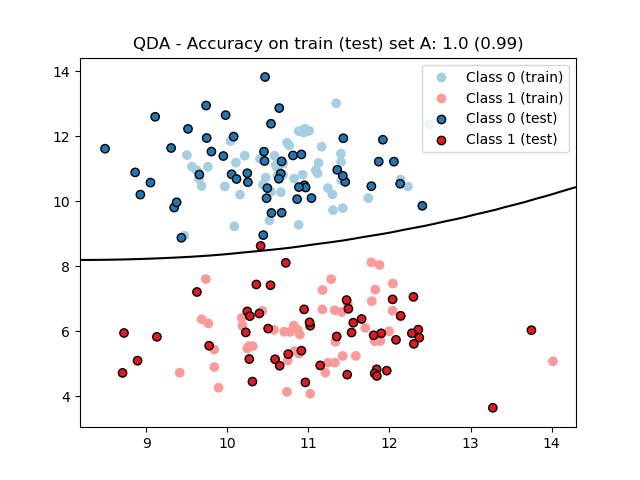
\includegraphics[width=\linewidth]{./images/QDA_A.png}
          \label{fig:qda_a}
        \endminipage\hfill
        \minipage{0.5\textwidth}
          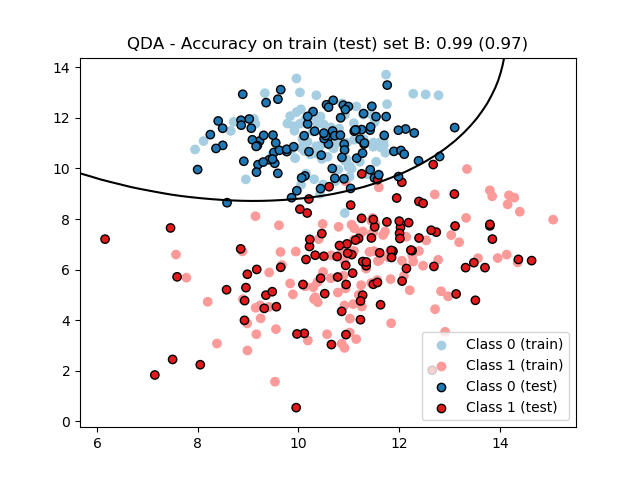
\includegraphics[width=\linewidth]{./images/QDA_B.png}
          \label{fig:qda_b}
        \endminipage\hfill
        \minipage{0.5\textwidth}%
          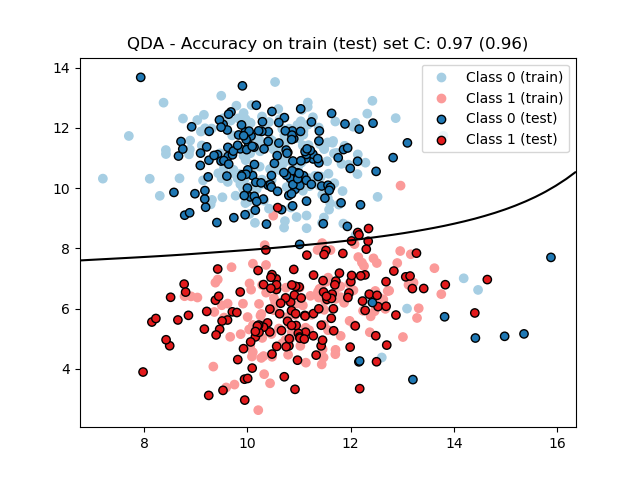
\includegraphics[width=\linewidth]{./images/QDA_C.png}
          \label{fig:qda_c}
        \endminipage
        \caption{The conics are defined by the equation $p(y=1|x)=0.5$ for the QDA Model.}
        \label{fig:qda-plot}
        \end{figure}
        
    \item Here are the results obtained with the QDA model: \\
    
    \begin{tabular}{ | l | *{3}{| c} | }
         \hline
            Misclassif. error & Dataset A & Dataset B & Dataset C \\
         \hline
           Train set & 0    & 0.01 & 0.03 \\
           Test set  & 0.01 & 0.03 & 0.04 \\
         \hline
     \end{tabular}
     
     \item We see that in most of the cases, the QDA performs better on the datasets B and C. As it seems that the datasets $B$ and $C$ are generated from two Gaussians with different means and different covariance matrices (with noisy examples for the dataset $C$), QDA model is well adapted. For the dataset A, it is not useful, as the data are linearly separable.
\end{enumerate}

\end{document}